% --------------------------------------------------------------
% This is all preamble stuff that you don't have to worry about.
% Head down to where it says "Start here"
% --------------------------------------------------------------
 
\documentclass[12pt]{article}
 
\usepackage[margin=1in]{geometry} 
\usepackage{amsmath,amsthm,amssymb}
 \usepackage{graphicx}
\newcommand{\N}{\mathbb{N}}
\newcommand{\Z}{\mathbb{Z}}
 
\newenvironment{theorem}[2][Theorem]{\begin{trivlist}
\item[\hskip \labelsep {\bfseries #1}\hskip \labelsep {\bfseries #2.}]}{\end{trivlist}}
\newenvironment{lemma}[2][Lemma]{\begin{trivlist}
\item[\hskip \labelsep {\bfseries #1}\hskip \labelsep {\bfseries #2.}]}{\end{trivlist}}
\newenvironment{exercise}[2][Exercise]{\begin{trivlist}
\item[\hskip \labelsep {\bfseries #1}\hskip \labelsep {\bfseries #2.}]}{\end{trivlist}}
\newenvironment{reflection}[2][Reflection]{\begin{trivlist}
\item[\hskip \labelsep {\bfseries #1}\hskip \labelsep {\bfseries #2.}]}{\end{trivlist}}
\newenvironment{proposition}[2][Proposition]{\begin{trivlist}
\item[\hskip \labelsep {\bfseries #1}\hskip \labelsep {\bfseries #2.}]}{\end{trivlist}}
\newenvironment{corollary}[2][Corollary]{\begin{trivlist}                      
\item[\hskip \labelsep {\bfseries #1}\hskip \labelsep {\bfseries #2.}]}{\end{trivlist}}
\newenvironment{definition}[2][definition]{\begin{trivlist}                      
\item[\hskip \labelsep {\bfseries #1}\hskip \labelsep {\bfseries #2.}]}{\end{trivlist}}
 
\begin{document}
 
% --------------------------------------------------------------
%                         Start here
% --------------------------------------------------------------
 
%\renewcommand{\qedsymbol}{\filledbox}
 
\title{Homework \#4}%replace X with the appropriate number
\author{Tanner Hammond\\ %replace with your name
CPSC 395 - Analysis of Algorithms
\\ Due: Monday, 8} %if necessary, replace with your course title
\date{}
\maketitle

\begin{enumerate}
\item Exercise 7.1-3 \\
Give a brief argument that the running time of PARTITION on a subarray of size n is $\Theta(n)$. \\
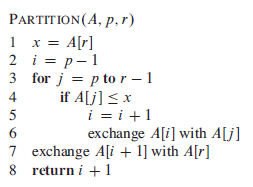
\includegraphics[scale=1]{Partition.png}

In the Partition algorithm and its parameters, A is an array of size n, p is the first index and r is the last index. Lines 1 and 2 are constant time statements so they're just O(1). From the conditions of the for loop, the for loop (lines 3-6) runs r-1-p times. The size of the array is r-p = n so the for loop is $\Theta(n)$ since it's proportional to the size. The statements inside the for loop (lines 4-6) all take constant time so they are also O(1). Line 7 and 8 are also both constant time. Everything is constant time except the for loop, so the running time of Partition for a subarray of size n is $\Theta(n)$.

\item Exercise 7.2-1 \\
Use the substitution method to prove that the recurrence T(n) = T(n-1) + $\Theta(n)$ has the solution T(n) = $\Theta(n^2)$ as claimed at the beginning of Section 7.2. \\
Using the substitution method as seen in 4.3, there are 2 steps: Guess the form of the solution and using mathematical induction to find the constants and show that the solution works. \\

T(n) = T(n-1) + $\Theta(n)$ We guess that the solution is T(n) = $\Theta(n^2)$. \\

Note: I had some difficulty with the substitution and being able to explain the steps I was taking so I'm going to go back to the chapter, reread and do some exercises. If I still feel like I'm having trouble I will set up an appointment.

\item Exercise 7.2-2 (Justify your answer) \\
What is the running time of QUICKSORT when all elements of array A have the same value? \\

There is an array of size n, where for p and r of the array p < r, and all of the contents are the same value. This also means the array is already sorted. The call to partition will have to go through the entire array so this will be the worst case runtime for Partition and will return q=r. The Partition will produce 2 sub problems, one containing n-1 items and the other 0.

\item Exercise 7.3-1 \\
Why do we analyze the expected running time of a randomized algorithm and not its worst-case running time? \\

Random algorithms better represent the typical runtime of an algorithm. Such as in quicksort, with the randomized partition we are more likely to see a better balance on average. The running time of a randomized algorithm isn't just dependent on the input but also the randomized choices that will happen in the algorithm.

\end{enumerate}
 

% --------------------------------------------------------------
%     You don't have to mess with anything below this line.
% --------------------------------------------------------------
 
\end{document}